Textual description of the dispute is preferably called as
\textit{Factual Aspect} in WTO DSB.
Since Panel
always provide a factual aspect\footnote{
  It's worth noting that Appellate Body doesn't provide any factual aspect because they always use the factual aspect provided by the Panel.
}
that describes the circumstances of the dispute
in each report, %(Figure \ref{fig:panel-report-toc}),
I wrote a program that
automatically search and collect
the Panel reports from the WTO official document website\footnote{
  \url{http://docs.wto.org}
}.
Then I located the factual aspect using the page information from the
table of contents in each Panel report as shown in Figure \ref{fig:panel-report-toc}.
I collected the total 143 numbers of different factual aspects . The collected case numbers are listed in Figure \ref{fig:ds-cases-used}.

\subsubsection{Joint Adjudication \& Early Settlement}
The number 143 may seem small compared to the total 596\footnote
{As of November 1st, 2020.} number of cases that are requested to WTO DSB. This is due to the following two reasons.
First, Panel jointly adjudicates different cases together if the cases raise the claim toward the
same trade policy of the same member state. For example, in \textit{US - Offset (Byrd Amendment)}, Panel merged DS217\footnote{
  DS refers to \textit{Dispute Settelement}. DS is the official prefix that indicates the case in WTO DSB.
} and DS234 together because they were asking the judicial opinion for the same government measure of the United States as shown in Figure \ref{fig:linked-cases}.
This paper selects the smallest case number as a representative number for this case of joint adjudication.
For example, DS217 and DS234 share the same Panel report then this paper chooses DS217 as a representative number as shown in Figure \ref{fig:ds-cases-used} where the list includes DS217 but not DS234.
Second, members sometimes find \textit{mutually agreeable solution} before the Panel expresses its judicial opinion by publishing its Panel report. Then Panel stops there and no factual aspect is provided. I omitted this kind of \textit{early settled} cases as well.
% \subsubsection{Judicial Economy \& Early Settlement}
\begin{figure}[t!]
  \begin{quote}
      DS 2,
      18,
      22,
      31,
      34,
      46,
      56,
      58,
      60,
      62,
      67,
      68,
      69,
      75,
      76,
      87,
      90,
      98,
      103,
      108,
      121,
      122,
      135,
      136,
      139,
      141,
      146,
      152,
      155,
      161,
      162,
      165,
      166,
      174,
      175,
      177,
      184,
      202,
      207,
      212,
      217,
      219,
      221,
      231,
      234,
      238,
      244,
      245,
      246,
      248,
      257,
      264,
      265,
      266,
      267,
      268,
      269,
      276,
      282,
      283,
      286,
      290,
      294,
      295,
      296,
      301,
      302,
      308,
      312,
      315,
      316,
      320,
      321,
      322,
      332,
      336,
      339,
      343,
      344,
      345,
      350,
      353,
      360,
      363,
      366,
      371,
      379,
      381,
      384,
      392,
      394,
      396,
      397,
      399,
      400,
      406,
      412,
      414,
      415,
      422,
      425,
      427,
      429,
      430,
      431,
      435,
      436,
      437,
      440,
      442,
      447,
      449,
      453,
      454,
      456,
      457,
      461,
      464,
      468,
      471,
      472,
      473,
      475,
      476,
      477,
      479,
      480,
      482,
      483,
      484,
      485,
      486,
      488,
      490,
      492,
      493,
      495,
      499,
      504,
      505,
      513,
      518,
      523
  \end{quote}
  \caption{
      \textbf{List of the Collected Case numbers:} ``DS + number'' uniquely identifies each dispute. For example, DS 523 refers to \textit{US — Pipe and Tube Products (Turkey)} where the United States was challenged by Turkey for its possibly inconsistent anti-dumping measure.
      % where Turkey claimed claimed possible illegal trade policy of United States on pipe ane tube products from Turk.
  }
  \label{fig:ds-cases-used}
\end{figure}
\begin{figure}[t!]
  \centering
  \frame{
    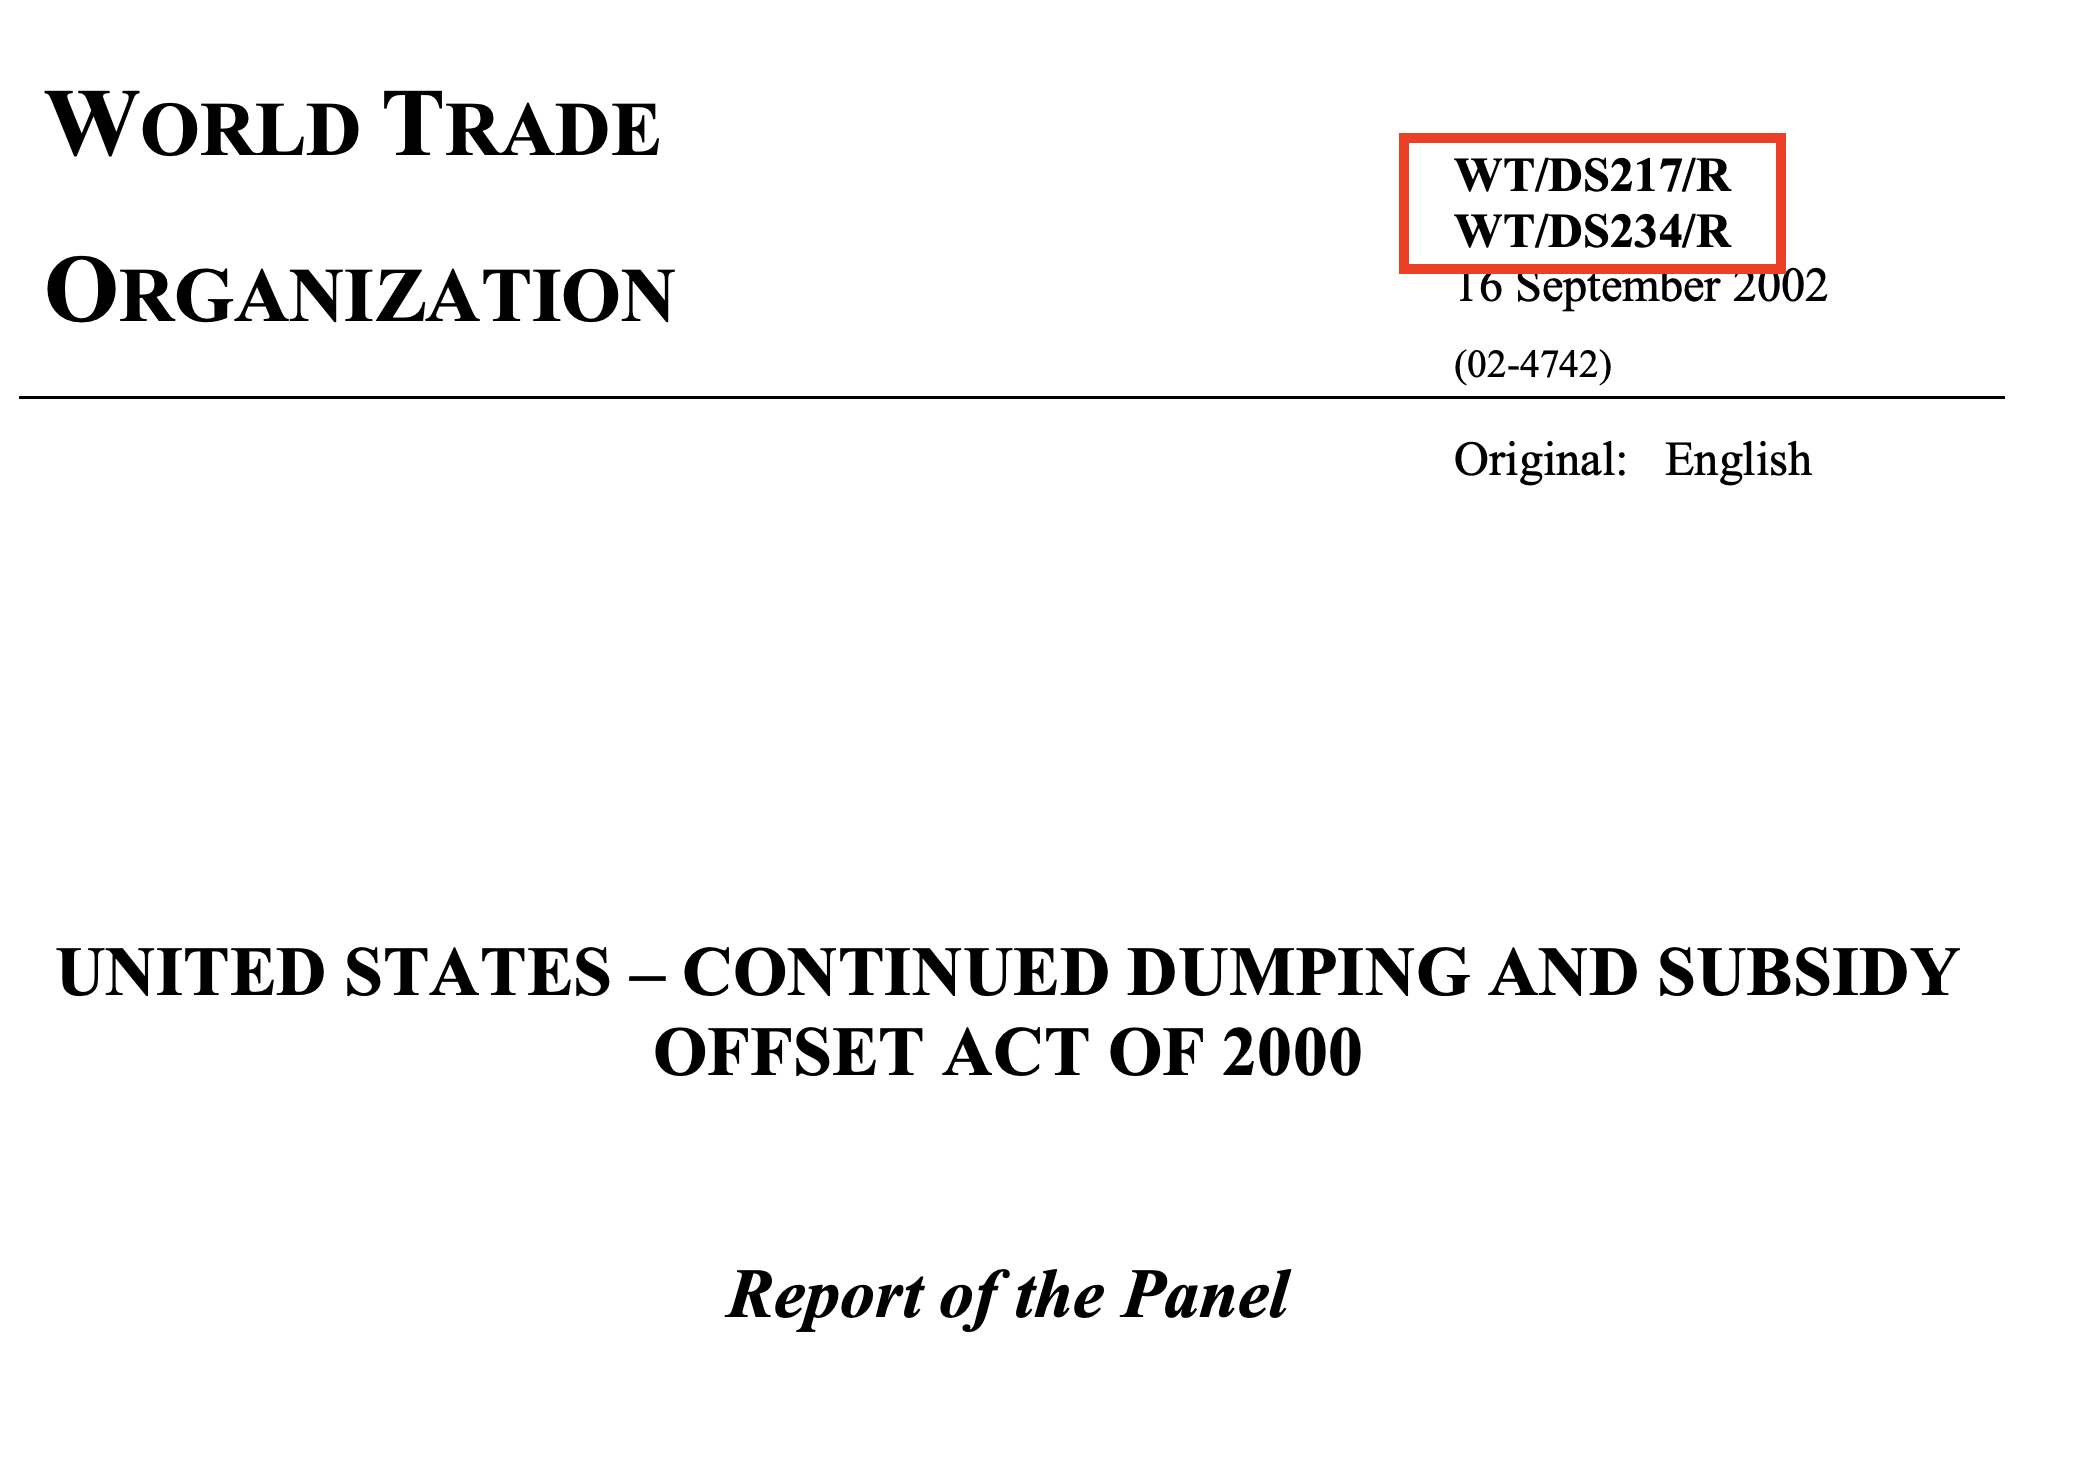
\includegraphics[scale=0.35]{Data/pngs/linked_cases.png}
  }
  \caption{\textbf{Cover of a Panel Report Includes Information about Joint Adjudication:}
      Panel explicitly marks which different cases are adjudicated together in the cover of the Panel report. DS217 and DS234 are handled together in this example.
      }
  \label{fig:linked-cases}
\end{figure}
% way before they express their
% legal conclusion as to the inconsistency  to the rules of the WTO or not.
% where the panel expresses
% its conclusion as to whether the challenged
% trade policy is inconsistent to the rules of the WTO or not.
 
 
 

